% This file was created with tikzplotlib v0.10.1.
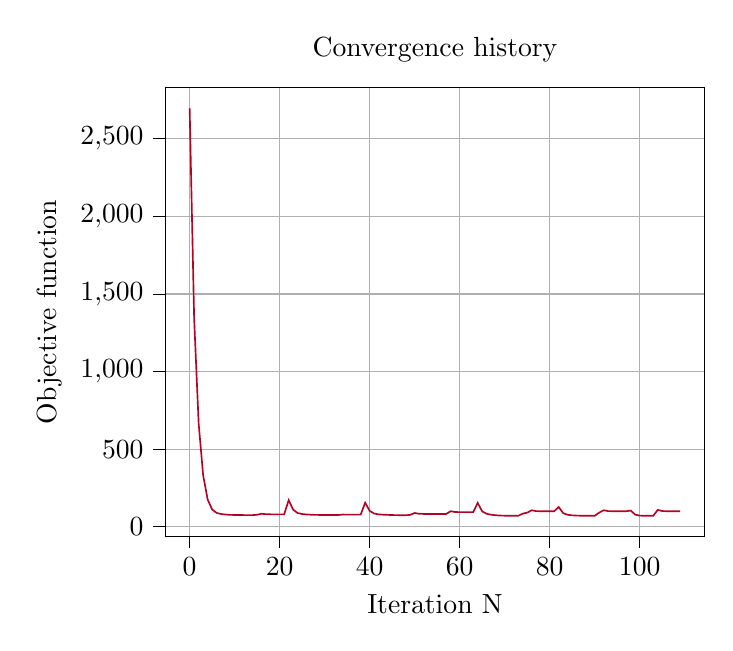
\begin{tikzpicture}

\definecolor{darkgray176}{RGB}{176,176,176}
\definecolor{firebrick180438}{RGB}{180,4,38}

\begin{axis}[
tick align=outside,
tick pos=left,
title={Convergence history},
x grid style={darkgray176},
xlabel={Iteration N},
xmajorgrids,
xmin=-5.45, xmax=114.45,
xtick style={color=black},
y grid style={darkgray176},
ylabel={Objective function},
ymajorgrids,
ymin=-61.0418325059019, ymax=2827.93105691617,
ytick style={color=black}
]
\addplot [semithick, firebrick180438]
table {%
0 2696.61410739698
1 1340.69719975026
2 665.295719944366
3 330.953397012819
4 175.94409133933
5 111.105831059072
6 89.0350154260762
7 81.7528610174375
8 78.4724355397695
9 76.5690624015191
10 75.6930548900034
11 75.2688746191894
12 75.0569196808242
13 74.9509416632314
14 74.8979513955702
15 77.1286339099154
16 83.6422082877931
17 80.4959121983754
18 79.8995252722031
19 79.8771090401021
20 79.8770766684397
21 79.877076668372
22 171.189929662957
23 109.970723629326
24 88.1860655261349
25 81.9841049576884
26 78.9226065036865
27 77.1878779563417
28 76.3861883067509
29 75.9290982919575
30 75.7005613117942
31 75.5862929278804
32 75.5291585181506
33 75.4915526926477
34 78.4042161518191
35 77.8207978253278
36 77.7819567706072
37 77.781861741352
38 77.7818617408375
39 154.884073558937
40 102.226210054953
41 84.917931986176
42 79.6744513119915
43 77.4702604358898
44 76.4752021462897
45 75.3042165387822
46 74.6095972917009
47 74.2657668184218
48 74.1273875625748
49 76.3893097850854
50 88.6043974151211
51 83.3738171439825
52 82.4449230658067
53 82.3497356108352
54 82.3148945111187
55 82.298774253138
56 82.2907252120884
57 82.2866992406658
58 99.9800512419565
59 94.7057658412309
60 94.136666847365
61 94.1298786727467
62 94.12987770661
63 94.12987770661
64 153.615639480245
65 98.5696813836095
66 83.3526469906861
67 77.4630121059889
68 73.9207736634879
69 72.06961517593
70 71.1215038581706
71 70.6338117600295
72 70.4099995400186
73 70.2983050274786
74 84.4854970798268
75 90.734553790847
76 106.00190070676
77 100.565352300636
78 99.9954062901105
79 99.988617894203
80 99.9886169282422
81 99.9886169282422
82 127.249603209753
83 87.3837668433433
84 76.8331513009711
85 73.3195711296095
86 71.741406384919
87 70.9570266932869
88 70.5562225227333
89 70.3712907720629
90 70.2789516535925
91 91.0102792272043
92 106.349175992854
93 100.581496454388
94 99.9954778360148
95 99.9886178962254
96 99.9886169282422
97 99.9886169282422
98 104.073794748997
99 77.894783212276
100 71.6127558839228
101 70.5432405027017
102 70.3637284027605
103 70.275117013283
104 108.702647765514
105 101.075354194844
106 100.011679856712
107 99.9887156132382
108 99.988616928254
109 99.9886169282422
};
\end{axis}

\end{tikzpicture}
